\documentclass[12pt,twoside]{article}
\usepackage[dvipsnames]{xcolor}
\usepackage{tikz,graphicx,amsmath,amsfonts,amscd,amssymb,bm,cite,epsfig,epsf,url}
\usepackage[hang,flushmargin]{footmisc}
\usepackage[colorlinks=true,urlcolor=blue,citecolor=blue]{hyperref}
\usepackage{amsthm,multirow,wasysym,appendix}
\usepackage{array,subcaption} 
% \usepackage[small,bf]{caption}
\newcommand{\red}[1]{{\leavevmode\color{red}{#1}}}
\newcommand{\blue}[1]{{\leavevmode\color{blue}{#1}}}
\usepackage{enumitem}


\makeatletter
\renewcommand*\env@matrix[1][*\c@MaxMatrixCols c]{%
  \hskip -\arraycolsep
  \let\@ifnextchar\new@ifnextchar
  \array{#1}}
\makeatother

\begin{document}

\begin{center}
{\large{\textbf{Final Review}} } \vspace{0.2cm}\\

\\
\end{center}
\section{ Lecture 1 vector spaces}
\begin{itemize}
    \item \mathbf{Vector Space }Definition (simplified - see notes)
A vector space consists of a set $V$ (whose elements are called vectors) and two operations $+$ and . such that
ㅍ. The sum of two vectors is a vector: for $\vec{x}, \vec{y} \in V$, the sum $\vec{x}+\vec{y}$ is a vector, i.e. $\vec{x}+\vec{y} \in V$.
ㄴ Multiplying a vector $\vec{x} \in V$ by a scalar $\lambda \in \mathbb{R}$ gives a vector $\lambda \cdot \vec{x} \in V$
" The operations + and · are "nice and compatible".
\item \mathbf{ Sub Space }Definition
We say that a non-empty subset $S$ of a vector space $V$ is a subspace if it is closed under addition and multiplication by a scalar, that is if
1. for all $x, y \in S$ we have $x+y \in S$,
2. for all $x \in S$ and all $\alpha \in \mathbb{R}$ we have $\alpha x \in S$.  
\item note that all subspaces are vector spaces
\item \mathbf{Span }Definition
Let $x_1, \ldots, x_k$ be vectors of $V$. We define the linear span of $x_1, \ldots, x_k$ as the set of all linear combinations of these vectors:
$$
\operatorname{Span}\left(x_1, \ldots, x_k\right) \stackrel{\text { def }}{=}\left\{\alpha_1 x_1+\cdots+\alpha_k x_k \mid \alpha_1, \ldots, \alpha_k \in \mathbb{R}\right\}
$$
\item \mathbf{Linearly Dependint }Vectors $x_1, \ldots x_k \in V$ are linearly dependent is there exists $\alpha_1, \ldots, \alpha_k \in \mathbb{R}$ that are not all zero such that
$$
\alpha_1 x_1+\cdots+\alpha_k x_k=0 .
$$
They are said to be linearly independent otherwise. Abuse of language: Instead of saying $« x_1, \ldots, x_k$ are linearly dependent», we should say «the family $\left(x_1, \ldots, x_k\right)$ is linearly dependent».
\item \mathbf{Bassis} Definition
A family $\left(x_1, \ldots, x_n\right)$ of vectors of $V$ is a basis of $V$ if\\
1. $x_1, \ldots, x_n$ are linearly independent,
\\2. $\operatorname{Span}\left(x_1, \ldots, x_n\right)=V$.
\\This means that $\left(x_1, \ldots, x_n\right)$ is a basis of $V$ if
\\1. None of the $x_i$ is a linear combination of the others $\left(x_j\right)_{j \neq i}$.
\\2. Any vector of $V$ can be expressed as a linear combination of $\left(x_1, \ldots, x_n\right)$.
\item \mathbf{Dimension}Theorem
Let $V$ be a vector space.
If $V$ admits a basis $\left(v_1, \ldots, v_n\right)$, then every basis of $V$ has also $n$ vectors. We say that $V$ has dimension $n$ and write $\operatorname{dim}(V)=n$.
" Otherwise, we say that $V$ has infinite dimension:
$
\operatorname{dim}(V)=+\infty \text {. }
$
\section{Lecture 2 matrcies and linear transforms}
\item \mathbf{Linear Transform }Definition
A function $L: \mathbb{R}^m \rightarrow \mathbb{R}^n$ is linear if
1. for all $v, w \in \mathbb{R}^m$ we have $L(v+w)=L(v)+L(w)$ and
2. for all $v \in \mathbb{R}^m$ and all $\alpha \in \mathbb{R}$ we have $L(\alpha v)=\alpha L(v)$.
\item \mathbf{Matrix} Consider a linear map $L: \mathbb{R}^m \rightarrow \mathbb{R}^n$ and its associated matrix $\widetilde{L} \in \mathbb{R}^{n \times m}$. where the columns of $\tilde{L}_i$ are $L(e_i)$ 
\item \mathbf{Kernel } The kernel $\operatorname{Ker}(L)$ (or nullspace) of $L$ is defined as the vectors $v \in \mathbb{R}^m$ such that $L(v)=0$, i.e.
$$
\operatorname{Ker}(L) \stackrel{\text { def }}{=}\left\{v \in \mathbb{R}^m \mid L(v)=0\right\}
$$
\item \mathbf{Image}
Definition (Image)
The image $\operatorname{Im}(L)$ (or column space) of $L$ is defined as the set of all vectors $u \in \mathbb{R}^n$ such that there exists $v \in \mathbb{R}^m$ such that $L(v)=u$.
\item \mathbf{solving systems} For an $A\in \mathbb{R}^{nXM}, x\in \mathbb{R}^N. y\in \mathbb{R}^m$ 
\\1. $y \notin \operatorname{Im}(A)$ : there is no solution to $A x=y$.
\\2. $y \in \operatorname{Im}(A)$, then there exists $x_0 \in \mathbb{R}^m$ such that $A x_0=y$. The set of solutions in then
$$
S=\left\{x_0+v \mid v \in \operatorname{Ker}(A)\right\} .
$$
\\$\therefore$ If $\operatorname{Ker}(A)=\{0\}$, then $S=\left\{x_0\right\}: x_0$ is the unique solution.
\\$\therefore$ If $\operatorname{Ker}(A) \neq\{0\}$, then $\operatorname{Ker}(A)$ contains infinitely many vectors: there are infinitely many solutions.
\section{Lecture 3 Rank }
\item \mathbf{Rank} Let $M \in \mathbb{R}^{n \times m}$. Let $r_1, \ldots, r_n \in \mathbb{R}^m$ be the rows of $M$ and $c_1, \ldots, c_m \in \mathbb{R}^n$ be its columns. Then we have
$
\operatorname{rank}\left(r_1, \ldots, r_n\right)=\operatorname{rank}\left(c_1, \ldots, c_m\right)=\operatorname{rank}(M)= Rank(M^t)=rank(M^TM)=rank(MM^T)
$

\item \mathbf{Rank Nullity} Let $L: \mathbb{R}^m \rightarrow \mathbb{R}^n$ be a linear transformation. and $L\in\mathbb{R}^{N^M}$Then 
$$
\operatorname{rank}(L)+\overbrace{\operatorname{dim}(\operatorname{Ker}}(L))=m .
$$
\item \mathbf{Inequalities} Let $A \in \mathbb{R}^{n \times m}$ and $B \in \mathbb{R}^{m \times k}$. Then the following holds
1. $\operatorname{rank}(A) \leq \min (n, m)$.
2. $\operatorname{rank}(A B) \leq \min (\operatorname{rank}(A), \operatorname{rank}(B))$.
Theorem
\item \mathbf{Invertability conditions }
Let $M \in \mathbb{R}^{n \times n}$. The following points are equivalent:
1. $M$ is invertible.
2. $\operatorname{rank}(M)=n$.
3. $\operatorname{Ker}(M)=\{0\}$.
4. For all $y \in \mathbb{R}^n$, there exists a unique $x \in \mathbb{R}^n$ such that $M x=y$.
\item $\operatorname{ker}(L)=\operatorname{ker}\left(L^{\top} L\right)$ for any $L \in \mathbb{R}^{n \times m}$
\section{Lecture 4 norms inner products and orthogonality}
\item \mathbf{euclidian norm } Definition
We define the Euclidean norm of $x=\left(x_1, \ldots, x_n\right) \in \mathbb{R}^n$ as:
$$
f(x)=\|x\|_2=\sqrt{x_1^2+\cdots+x_n^2} .
$$
\item \mathbf{Genearl Norm}
Let $V$ be a vector space.
Definition A norm $\|\cdot\|$ on $V$ is a function from $V$ to $\mathbb{R}_{>0}$ that verifies:
\\1. Homogeneity: $\|\alpha v\|=|\alpha| \times\|v\|$ for all $\alpha \in \mathbb{R}$ and $v \in V$.
\\ 2. Positive definiteness: if $\|v\|=0$ for some $v \in V$, then $v=0$.
\\ 3. Triangular inequality: $\|u+v\| \leq\|u\|+\|v\|$ for all $u, v \in V$.
\\Note that "norm" = "length" = "distance".

\item The L1 Norm $\|x\|_1 \stackrel{\text { def }}{=} \sum^n\left|x_i\right|=\left|x_1\right|+\cdots+\left|x_n\right| \text {. }$
\item Definition
We define the Euclidean dot product of two vectors $x$ and $y$ of $\mathbb{R}^n$ as:
$$
x \cdot y=\sum_{i=1}^n x_i y_i=x_1 y_1+\cdots+x_n y_n
$$
\item \mathbf{Genearl Inner Products } Let $V$ be a vector space.
Definition
An inner producton $V$ is a function $\langle\cdot, \cdot\rangle$ from $V \times V$ to $\mathbb{R}$ that verifies the following points:
\\1. Symmetry: $\langle u, v\rangle=\langle v, u\rangle$ for all $u, v \in V$.
\\2. Linearity: $\langle u+v, w\rangle=\langle u, w\rangle+\langle v, w\rangle$ and $\langle\alpha v, w\rangle=\alpha\langle v, w\rangle$ for all $u, v, w \in V$ and $\alpha \in \mathbb{R}$. $\quad\langle u+v, w\rangle=\sum_i\left(u_i+v_i\right) w_i=\sum_i u_i w_i$
\\3. Positive definiteness: $\langle v, v\rangle \geq 0$ with equality if and only if $+\sum_i v_i w_i$ $v=0$.
$$
=\left\langle u_1 \omega\right\rangle+\langle u, \omega\rangle
$$

\item \mathbf{Norm induced by inner product}
Proposition if  $\langle\cdot, \cdot\rangle$ is an inner product on $V$ 
$$
||v\| \stackrel{\text { def }}{=} \sqrt{\langle v, v\rangle} \text {. }
$$
is a norm on $V$. We say that the norm $\|\cdot\|$ is induced by the inner product $\langle\cdot, \cdot\rangle$.

\item \mathbf{Orthogonality} We say that vectors $x$ and $y$ are orthogonal if $\langle x, y\rangle=0$. We write then $x \perp y$
:We say that a vector $x$ is orthogonal to a set of vectors $A$ if $x$ is orthogonal to all the vectors in $A$. We write then $x \perp A$.


\item Definition
We say that a family of vectors $\left(v_1, \ldots, v_k\right)$ is:
\\$\because$ orthogonal if the vectors $v_1, \ldots, v_k$ are pairwise orthogonal, i.e. $\left\langle v_i, v_j\right\rangle=0$ for all $i \neq j$.
\\ : orthonormal if it is orthogonal and if all the $v_i$ have unit norm: $\left\|v_1\right\|=\cdots=\left\|v_k\right\|=1$.

\item \mathbf{Pythagoran therome } Theorem (Pythagorean theorem)
Let $\|\cdot\|$ be the norm induced by $\langle\cdot, \cdot\rangle$. For all $x, y \in V$ we have
$$
x \perp y \Longleftrightarrow\|x+y\|^2=\|x\|^2+\|y\|^2 .
$$

\item Definition
Let $S$ be a subspace of $\mathbb{R}^n$. The orthogonal projection of a vector $x$ onto $S$ is defined as the vector $P_S(x)$ in $S$ that minimizes the distance to $x$ :
$$
P_S(x) \stackrel{\text { def }}{=} \underset{y \in S}{\arg \min }\|x-y\| .
$$
The distance of $x$ to the subspace $S$ is then defined as
$$
d(x, S) \stackrel{\text { def }}{=} \min _{y \in S}\|x-y\|=\left\|x-P_S(x)\right\| .
$$
\item Proposition
Let $S$ be a subspace of $\mathbb{R}^n$ and let $\left(v_1, \ldots, v_k\right)$ be an orthonormal basis of $S$. Then for all $x \in \mathbb{R}^n$,
$$
P_S(x)=\left\langle v_1, x\right\rangle v_1+\cdots+\left\langle v_k, x\right\rangle v_k .
$$
\item \mathbf{Orthognal matrix} Let $V=\left(\begin{array}{ccc}\mid & & \mid \\ v_1 & \cdots & v_k \\ \mid & & \mid\end{array}\right)$ gather the orthonormal basis-vectors of the subspace $S$
Proposition
The orthogonal projection is given by $P_S(x)=V V^{\top} x$.
$=P_S$ is a linear transform.
$=V V^{\top}$ is its matrix.
\item consiquinces For all $x \in \mathbb{R}^n$,
\\$\because x-P_S(x)$ is orthogonal to $S$.\\
$\therefore\left\|P_S(x)\right\| \leq\|x\|$.
\section{lecture 5 orthogonal matrices}
\item from ghram schmit we see that every substance of $\mathbb{R}^N$ admits an orthonomral bassis, so the bassic point is we can turn the linearly independint row  or cols of any matrix into an abnormal bassis of that matrix or its transpose 
\item  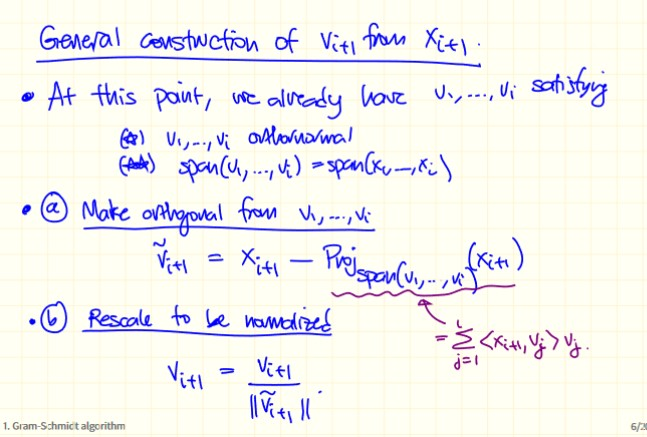
\includegraphics[width=10cm]{final Review/gm.jpg}
\item here is the ghram schmit process
\item \mathbf{Orthonomal matricies} a matrix is orthonormal if it is square and either its colomns or rows form an orthonormal family
\item  the following are all equivlent 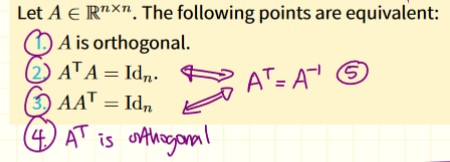
\includegraphics[width=10cm]{final Review/Orthognial equiv.jpg}
\item it is important to remember that orthogonal matrices are just rotations. this is $A^TA=AA^t=I$ meaning that tehy litterly have all eigen values one. so all they really do is change the bassis of a vector (which is effectively roate that vector but do not rescale them)
\item A vector x times an orthoginal matrix a yields the cordinates of that vector in the bassis of A that is A^{\top} x=\left[\begin{array}{c}
-a_1^{\top}- \\
\vdots \\
-a_n^{\top}-
\end{array}\right]\left[\begin{array}{c}
x_1 \\
\vdots \\
x_n
\end{array}\right]=\left[\begin{array}{c}
\left\langle a_1, x\right\rangle \\
\left\langle a_2, x\right\rangle \\
\vdots \\
\left\langle a_n, x\right\rangle
\end{array}\right]


\section{Lecture 6 Eigen Vectors }
\item \mathbf{Eigenvector defention }Let $A \in \mathbb{R}^{n \times n}$. A non-zero vector $v \in \mathbb{R}^n$ is said to be an eigenvector of $A$ is there exists $\lambda \in \mathbb{R}$ such that
$$
A v=\lambda v .
$$
The scalar $\lambda$ is called the eigenvalue (of $A$ ) associated to $v$.
\item keep in mind that in a geometric sense the eigen vectors of a matrix are those vectors that when multiplied by a matrix are not rotated and are instead just scaled. 
\item the identity matrix in $\mathbb{R}^n$ has eigen value 1 with multiplicity n
\itme the bass  of the kernel of any matrix are eigenvectors associated with 0. 
\item note that the rotation by theta matrix has no real eigen values  $R_\theta=\left(\begin{array}{cc}
\cos \theta & -\sin \theta \\
\sin \theta & \cos \theta
\end{array}\right) \quad \text { for } \theta \in(0, \pi) $
\item the orthogonal projection matrix onto a subspace S, which can be expressed as the product of orthogonal matrices $V^TV$ has all vectors in s as eigen vectors asociated to 1,  and all vectors orthogonal to x as eigenvectors asociated to 0. 
\item FACT I: For $\alpha \in \mathbb{R} \quad \alpha \lambda$ is an eigenvalue of $\alpha A$ with iigarector $x$
\item FACT II: For $\alpha \in \mathbb{R}, \quad \alpha+\lambda$ is an eigen value of the matrix $A+\alpha I d$ with eigen vector $x$
\item Fact 3
For all $k \in \mathbb{N}, \lambda^k$ is an eigenvalue of the matrix $A^k$ and $x$ is an associated eigenvector.
\item Fact 4
If $A$ is invertible then $1 / \lambda$ is an eigenvalue of the matrix inverse $A^{-1}$ and $x$ is an associated eigenvector.
\item eigensapce defetnion Definition
If $\lambda \in \mathbb{R}$ is an eigenvalue of $A \in \mathbb{R}^{n \times n}$, the set
$$
E_\lambda(A)=\left\{x \in \mathbb{R}^n \mid A x=\lambda x\right\}=\operatorname{Ker}\left(\mathrm{A}-\lambda I_d\right)
$$
is called the eigenspace of $A$ associated to $\lambda$. The dimension of $E_\lambda(A)$ is called the multiplicity of the eigenvalue $\lambda$.
\item the spectrum of A is the set of the eigenvectors of A, the specturm of a must be less than the rank of A,
\item the sum of the multiplcites of the eigenvector of A equal n for a nxn square matirx 
\item 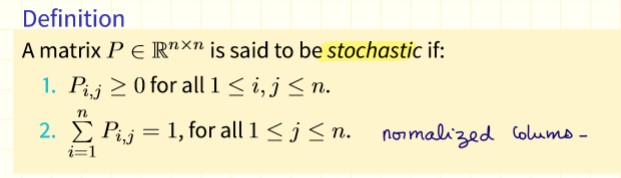
\includegraphics[width=10cm]{final Review/stochastic def.jpg}
\item there were not clearly written out defentions of things but a lot of the objecys in markov chains are implictly defined here 
\item 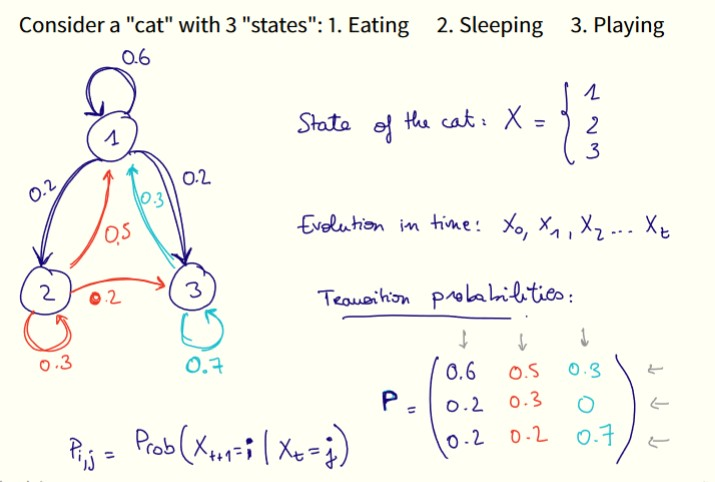
\includegraphics[width=15cm]{final Review/markov chain defentions .jpg}
\item 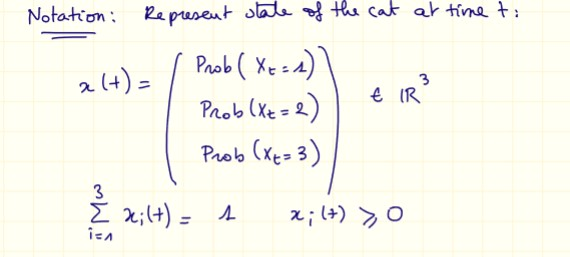
\includegraphics[width=10cm]{final Review/state vector.jpg}
\item 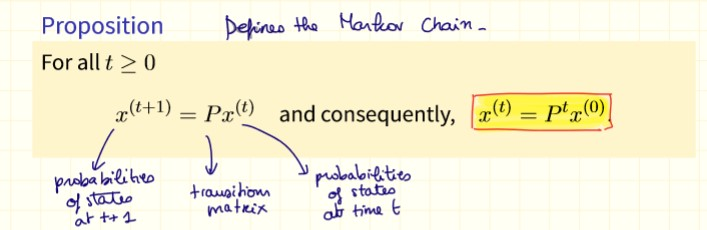
\includegraphics[width=10cm]{final Review/long term .jpg}
\item 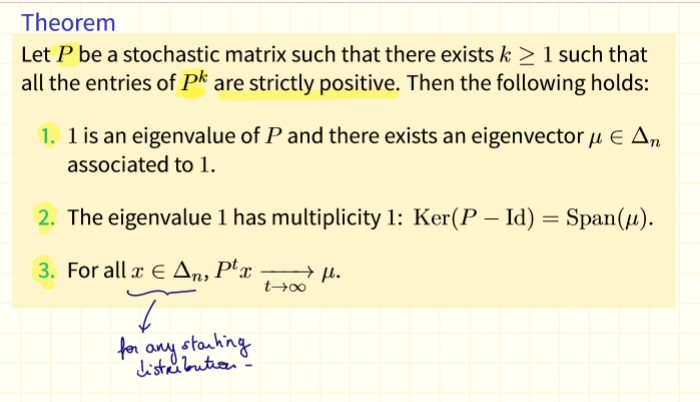
\includegraphics[width=10cm]{final Review/long term 2 .jpg}

\item Problem 6.2 (4 points). Let $v \in \mathbb{R}^n$ be a non-zero vector. What are the eigenvalues of the $n \times n$ matrix $M=v v^T$ ? What are the multiplicities of these eigenvalues? Justify.
\item sollution Answer 6.2. Observe that $M v=v v^T v=\|v\|^2 v$. Thus $v$ is an eigenvector of $M$ with eigenvalue $\lambda=\|v\|^2$. (Note that this $\lambda \neq 0$ since $v \neq 0$.) Thus $\|v\|^2$ is an eigenvalue with multiplicity at least 1. Observe also that for any vectors $x \in \operatorname{Span}(v)^{\perp}, M x=v v^T x=\langle x, v\rangle v=0$. Thus 0 is an eigenvalue of $M$ with multiplicity at least $\operatorname{dim}\left(\operatorname{Span}(v)^{\perp}\right)=n-\operatorname{dim}(\operatorname{Span}(v))=n-1$. By the proposition in lecture that the sum of multiplicities over all eigenvalues is at most $n$, we conclude that $M$ has eigenvalues 1 and 0 with multiplicities 1 and $n-1$, respectively.


\section{lecture 7 Spectral Therome  and PCA }
\item 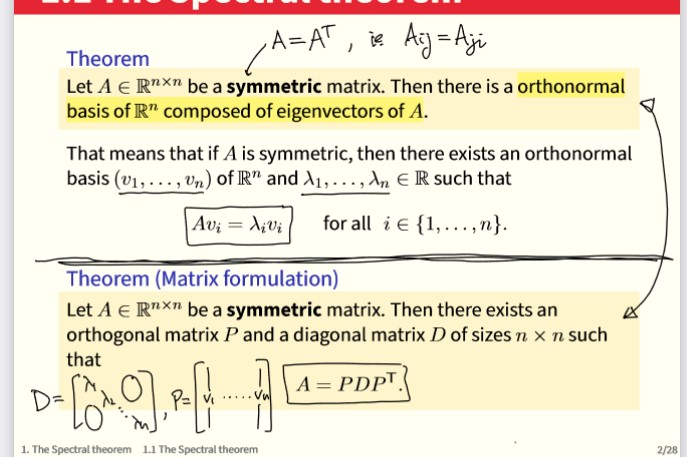
\includegraphics[width=15cm]{final Review/spectral.jpg}
\item this more or less means that any square symetric matrix A can be expressed using two orthomial matrcies that hold it's eigenvectors and a daignol matrix that holds is eigen values 
\item so when we multiply A times a vecor x what happens is $P^tx$ transofms x to be in teh bassis of a  (ie rotates X) $DP^tx$ rescalles x by the eigenveoctors of A, then finally $A(DP^tx)$ returns the ressults to the orginal bassis of x. 
\item Consequence \#1: $\lambda_1, \ldots, \lambda_n$ are the only eigenvalues of $A$, and the number of time that an eigenvalue appear on the diagonal equals its multiplicity.
\item 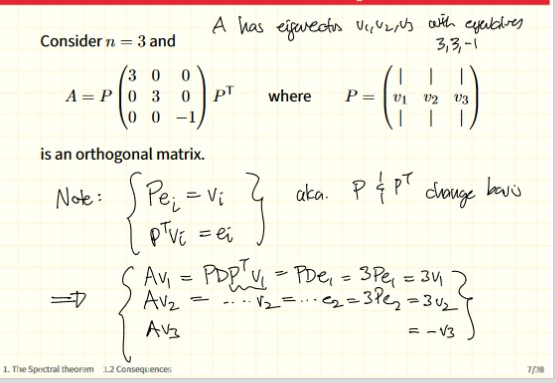
\includegraphics[width=15cm]{final Review/spectral example.jpg}
\item consiquince 2 the rank of a is equla to the number of non zdro enteries in d 
\item Consequence \#3: $\left[A\right.$ is invertible if and only if $\lambda_i \neq 0$ for all $\left.i.\right]$ In such case
$$
A^{-1}=P\left(\begin{array}{cccc}
1 / \lambda_1 & 0 & \cdots & 0 \\
0 & 1 / \lambda_2 & & \vdots \\
\vdots & & \ddots & 0 \\
0 & \cdots & 0 & 1 / \lambda_n
\end{array}\right) P^{\top}
$$
\item i am just going to print out the rest of lecture 7 through 12 

\section{cool questions }
\item 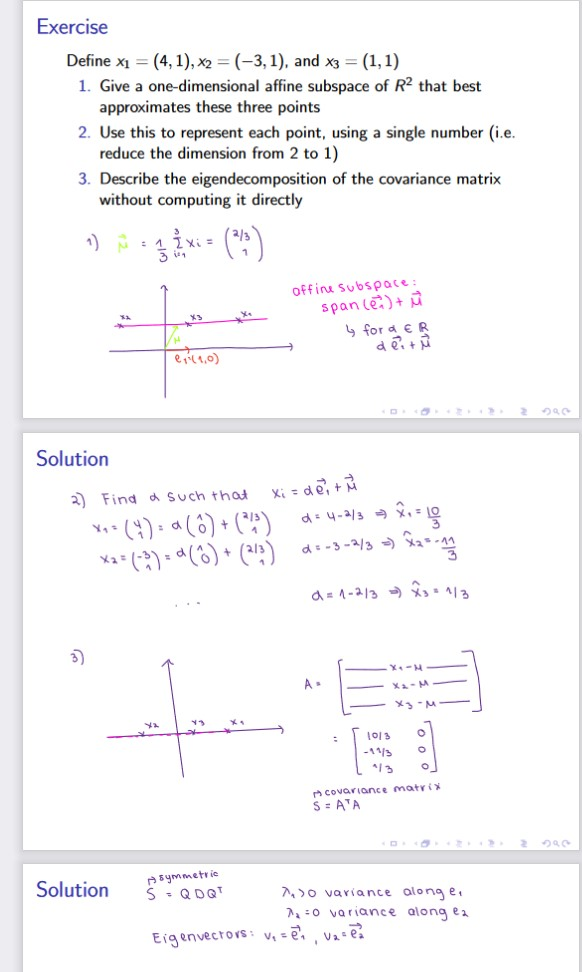
\includegraphics[width=15cm]{final Review/lab 7 excercise 3 .jpg}
\item 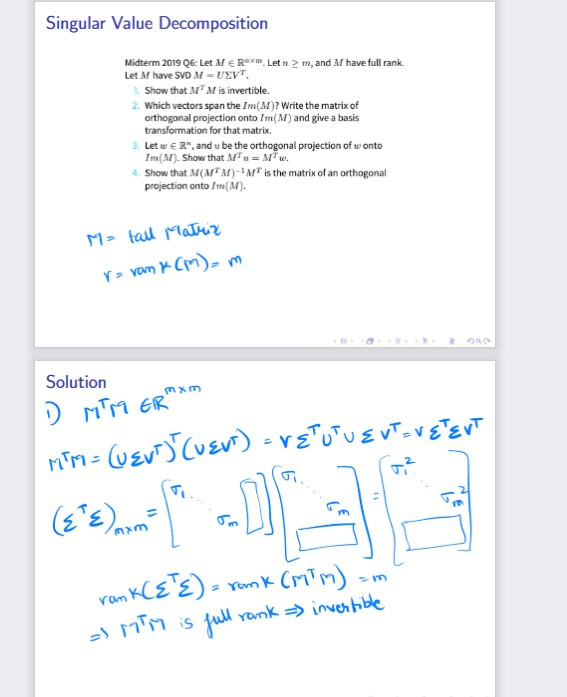
\includegraphics[width=15cm]{final Review/lab 8 part 1 .jpg}
\item 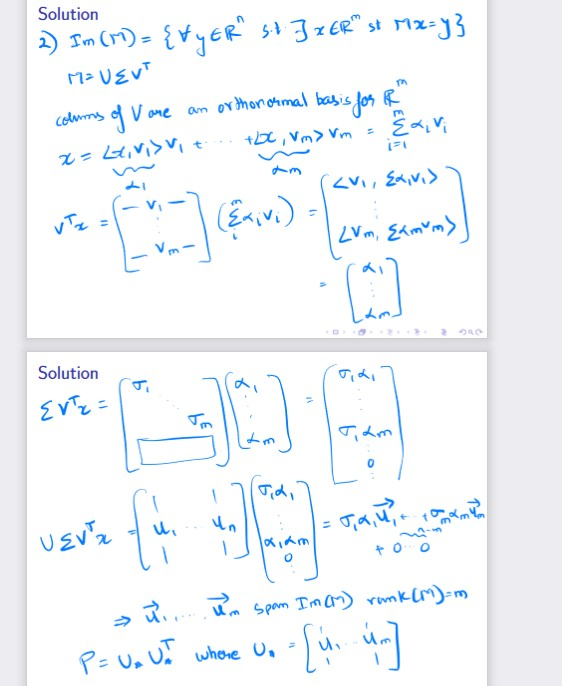
\includegraphics[width=15cm]{final Review/lab 8 part 2 .jpg}
\item 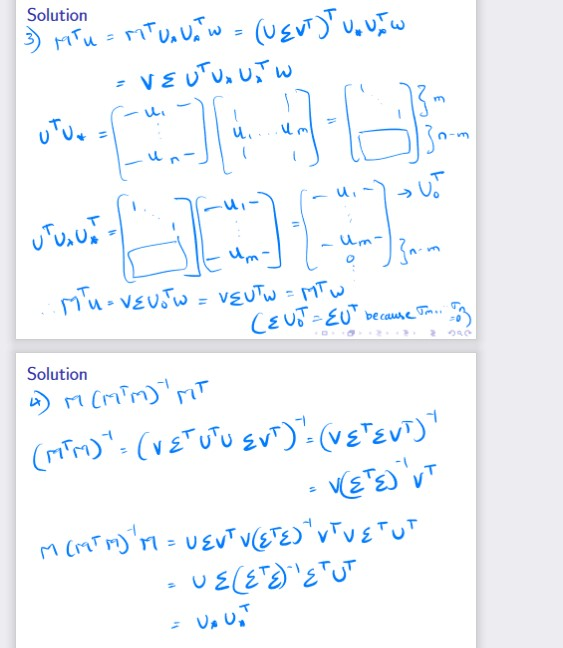
\includegraphics[width=15cm]{final Review/lab 8 part 3 .jpg}
\end{itemize}
\end{document}
